%-------------------------------------------------------------------------------
%-------------------------------------------------------------------------------
%-------------------------------------------------------------------------------
\chapter{DS4 : Centrale 2015}
%-------------------------------------------------------------------------------
%-------------------------------------------------------------------------------
%-------------------------------------------------------------------------------
\section{Graphes d'intervalles}
%-------------------------------------------------------------------------------
%-------------------------------------------------------------------------------
%-------------------------------------------------------------------------------
On considère le problème concret suivant : des cours doivent avoir
lieu dans un intervalle de temps précis (de 8h à 9h55, \dots), et on cherche à
attribuer une salle à chaque cours. On souhaite qu'à tout moment une
salle ne puisse être attribuée à deux cours différents et on aimerait
utiliser le plus petit nombre de salles possibles.

Ce problème d'allocation de ressources (ici les salles) en fonction de
besoins fixes (ici les horaires des cours) intervient dans de
nombreuses situations très diverses (allocation de pistes
d'atterrissage aux avions, répartition de la charge de travail sur
plusieurs machines, \dots).
%-------------------------------------------------------------------------------
%-------------------------------------------------------------------------------
\subsection{Représentation du problème}
%-------------------------------------------------------------------------------
%-------------------------------------------------------------------------------
On modélise le problème ainsi :
\begin{itemize}
\item chaque besoin est représenté par un segment $[a; b]$ où
  $a,b\in \N$ et $a\le b$.
\item deux besoins $I$ et $J$ sont en conflit quand $I\cap J\ne
  \emptyset$.
\end{itemize}

La donnée du problème est une suite finie $(I_0,\dots,I_{n-1})$ de $n$ segments où $n\in \N$.

%--------------------------------------------------------------------------
\begin{figure}[ht]
\centering
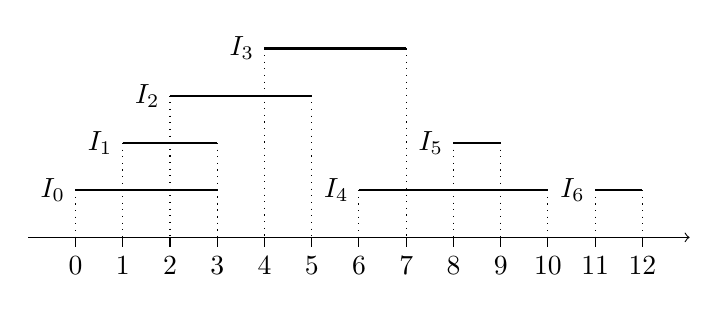
\begin{tikzpicture}[scale=0.6]
\draw[->](-1, 0) -- (13,0);
\foreach \i in {0, 1, 2, ..., 12}
    \draw (\i, 0.) -- (\i, -0.2) node[below]{$\i$};
\foreach \k/\a/\b/\h in {0/0/3/1, 1/1/3/2, 2/2/5/3, 3/4/7/4, 4/6/10/1, 5/8/9/2, 6/11/12/1}
    {\draw[thick] (\a, \h) node[left]{$I_{\k}$} -- (\b, \h);
     \draw[dotted] (\a, \h) -- (\a, 0);
     \draw[dotted] (\b, \h) -- (\b, 0);};     
\end{tikzpicture}
\caption{\label{fig:pba}Problème (a)}
\end{figure} 
%-------------------------------------------------------------------------------
On représente un segment en Caml par un couple d'entiers, la donnée du
problème est une valeur du type \type{(int*int) array}. Le problème (a) de
la figure \ref{fig:pba} est représenté par le tableau
\begin{lstlisting}
[|(0,3); (1,3); (2,5); (4,7); (6,10); (8,9); (11,12)|]
\end{lstlisting}
%-------------------------------------------------------------------------------
%-------------------------------------------------------------------------------
\begin{Exercise}\it
Écrire une fonction \type{conflit} telle que \type{conflit I J}
renvoie \type{true} si et seulement si $I$ et $J$ sont en conflit.
\end{Exercise}  
%-------------------------------------------------------------------------------
\begin{lstlisting}
conflit : int * int -> int * int -> bool
\end{lstlisting}
%-------------------------------------------------------------------------------
\begin{Answer}
Il y a conflit entre $[a;b]$ et $[c;d]$ lorsqu'il existe $x\in [a;b] \cap [c;d]$ ; cela implique $a \le x \le d$ et $c \le x \le b$.

Inversement si on a $a \le d$ et $c \le b$ alors,
\begin{itemize}
    \item soit $c\le a$, alors $a\in [c;d]$ car on a $a\le d$,
    \item soit $c > a$ donc $a < c \le b$ d'où $c\in [a;b]$.
\end{itemize}
Il y a donc conflit si et seulement si $a \le d$ et $c \le b$.

\begin{lstlisting}
let conflit (a, b) (c, d) = (c <= b) && (a <= d);;
\end{lstlisting} 
\end{Answer}
%-------------------------------------------------------------------------------
%-------------------------------------------------------------------------------
\subsection{Graphe d'intervalles}
%-------------------------------------------------------------------------------
%-------------------------------------------------------------------------------
À toute suite finie de segments, $\overline{I}=(I_0,\dots,I_{n-1})$ on associe un graphe non orienté, le {\bf graphe d'intervalles} $G\bigl(\overline I\bigr)=(S, A)$
\begin{itemize}
\item dont les sommets sont les segments $I_k$, $0\le k< n$,
\item où, pour $i,j\in \{0,\dots,n-1\}$ avec $i\ne j$, $(I_i, I_j)$ et $(I_j, I_i)$ sont des arêtes (on dit que $I_i$ et $I_j$ sont reliés) si et seulement si $I_i$ et $I_j$ sont en conflit.
\end{itemize}
Le graphe d'intervalles qui correspond au problème a admet la représentation graphique suivante.
%--------------------------------------------------------------------------
\begin{center}
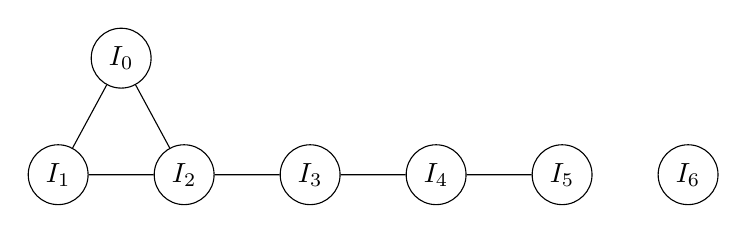
\begin{tikzpicture}[scale=0.8]
\foreach \k in {1, 2, ...,6}
    \draw ({2*\k}, 0) node[draw,fill=white, circle] (I\k) {$I_\k$};
\draw (3, 1.85) node[draw,fill=white, circle] (I0) {$I_0$};
\draw (I2) -- ( I0) -- (I1) -- (I2) -- (I3) -- (I4) -- (I5);
\end{tikzpicture}
\end{center} 
%-------------------------------------------------------------------------------
%-------------------------------------------------------------------------------
\begin{Exercise}\it
Donner une représentation graphique du graphe d'intervalles pour le problème (b) de la figure \ref{fig:pbb}.
\end{Exercise}  
%-------------------------------------------------------------------------------
\begin{Answer}
\begin{center}
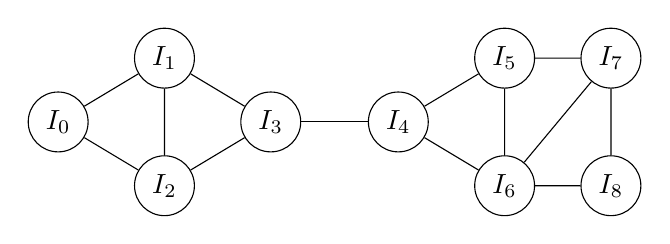
\begin{tikzpicture}[scale=0.27]
\foreach \k/\x/\y in {0/0/0, 1/5/3, 2/5/-3, 3/10/0, 4/16/0, 5/21/3, 6/21/-3, 7/26/3, 8/26/-3}
    \draw (\x, \y) node[draw,fill=white, circle] (I\k) {$I_\k$};
\foreach \i/\j in {0/1, 0/2, 1/2, 1/3, 2/3, 3/4, 4/5, 4/6, 5/6, 5/7, 6/7, 6/8, 7/8}
    \draw (I\i) -- (I\j);
\end{tikzpicture}
\end{center} 
\end{Answer}
%-------------------------------------------------------------------------------
%-------------------------------------------------------------------------------
\begin{figure}[ht]
\centering
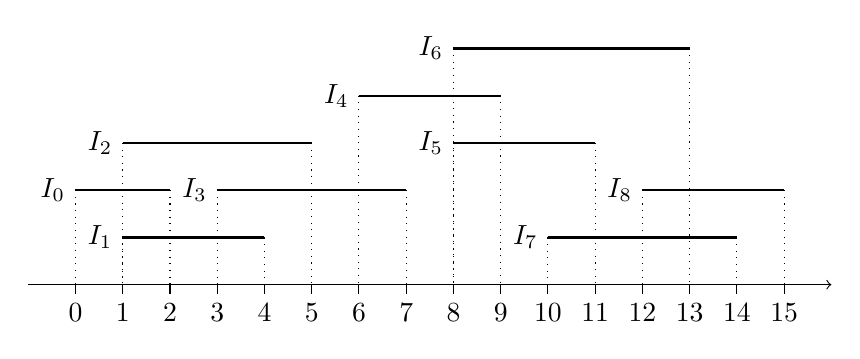
\begin{tikzpicture}[scale=0.6]
\draw[->](-1, 0) -- (16,0);
\foreach \i in {0, 1, 2, ..., 15}
    \draw (\i, 0.) -- (\i, -0.2) node[below]{$\i$};
\foreach \k/\a/\b/\h in {0/0/2/2, 1/1/4/1, 2/1/5/3, 3/3/7/2, 4/6/9/4, 
                         5/8/11/3, 6/8/13/5, 7/10/14/1, 8/12/15/2}
    {\draw[thick] (\a, \h) node[left]{$I_{\k}$} -- (\b, \h);
     \draw[dotted] (\a, \h) -- (\a, 0);
     \draw[dotted] (\b, \h) -- (\b, 0);};     
\end{tikzpicture}
\caption{\label{fig:pbb}Problème (b)}
\end{figure} 
%-------------------------------------------------------------------------------
Un graphe est implémenté par le tableau \type{g} de listes d'adjacence, de type \type{int list array}, où \type{g.(i)} est une liste contenant les entiers \type{j} tels que $I_j$ est relié à $I_i$..

Par exemple le problème (a) donne un graphe implémenté par 
\begin{lstlisting}
[|[1; 2; 3] ; [0; 2; 3] ; [0; 1; 3; 4] ; [0; 1; 2] ; [2]|]
\end{lstlisting}
%-------------------------------------------------------------------------------
%-------------------------------------------------------------------------------
\begin{Exercise}\it
Écrire une fonction \type{construit\_graphe} qui, étant donné un problème $\overline I$, renvoie la représentation de $G\bigl(\overline I\bigr)$ où les intervalles sont numérotés par leur ordre dans le tableau.
\end{Exercise}  
%-------------------------------------------------------------------------------
\begin{lstlisting}
construit_graphe : int * int array -> int list array
\end{lstlisting}
%-------------------------------------------------------------------------------
\begin{Answer}
Il suffit de balayer tous les couples $(i,j)$ avec $0 \le i < j \le n-1$.
\begin{lstlisting}
let construit_graphe seg =
   let n = Array.length seg in
   let g = Array.make n [] in
   for i = 0 to (n-2) do
      for j = (i+1) to (n-1) do
         if conflit seg.(i) seg.(j)
         then begin g.(i) <- j::g.(i); 
                    g.(j) <- i::g.(j) end done done;
   g;;
\end{lstlisting}
\end{Answer}
%-------------------------------------------------------------------------------
\newpage
%-------------------------------------------------------------------------------
\subsection{Coloration}
%-------------------------------------------------------------------------------
%-------------------------------------------------------------------------------
Une {\bf coloration} d'un graphe non orienté $G = (S, A)$ avec $S = (x_0, x_1, \ldots, x_{n-1})$ est une suite $(c_0, c_1, \ldots, c_{n-1})$ telle que $c_i \ne c_j$ pour toute arête $(x_i, x_j)$.

Par exemple $(0, 1, 2, 3, 0, 1, 0)$ est une coloration du graphe du problème (a).

L'entier $c_i$ est appelé la couleur du sommet $x_i$ et la condition se traduit ainsi : deux sommets reliés ont des couleurs distinctes. Dorénavant, le terme couleur sera synonyme d'entier naturel.

\medskip

Une coloration qui utilise le plus petit nombre de couleurs distinctes possibles, est dite {\bf optimale}. Ce nombre minimum de couleurs est noté $\chi(G)$, c'est le {\bf nombre chromatique} de $G$.

En associant une salle à chaque couleur, on peut répondre au problème initial à l'aide d'une coloration de son graphe d'intervalles associé.
%-------------------------------------------------------------------------------
%-------------------------------------------------------------------------------
\begin{Exercise}\it
Déterminer des colorations optimales pour les graphes d'intervalles associés aux deux problèmes (a) et (b). On attribuera à chaque fois la couleur $0$ à l'intervalle $I_0$
\end{Exercise}  
%-------------------------------------------------------------------------------
\begin{Answer}
Dès qu'il y a conflit il faut au moins deux couleurs.
S'il existe un cycle de 3 sommets dans le graphe alors il faut au moins 3 couleurs.

Les deux graphes demandent donc au moins 3 couleurs.

3 couleurs suffisent avec, par exemple,
\begin{itemize}
\item la coloration (0, 1, 2, 0, 1, 0, 0) pour le problème (a) et
\item la coloration (0, 1, 2, 0, 1, 0, 2, 1, 0) pour le problème (b).
\end{itemize}
\end{Answer}
%-------------------------------------------------------------------------------
%-------------------------------------------------------------------------------
\begin{Exercise}\it
Écrire une fonction \type{appartient} telle que l'appel \type{appartient l x} renvoie \type{true} si et seulement si l'entier $x$ est présent dans la liste \type{l}.
\end{Exercise}  
%-------------------------------------------------------------------------------
\begin{lstlisting}
appartient : int list -> int -> bool
\end{lstlisting}
%-------------------------------------------------------------------------------
\begin{Answer}
Un grand classique \dots
\begin{lstlisting}
let rec appartient liste x =
   match liste with
   |[] -> false
   |t::q -> (t = x) || (appartient q x);;
\end{lstlisting}
\end{Answer}
%-------------------------------------------------------------------------------
%-------------------------------------------------------------------------------
\begin{Exercise}\it
Écrire une fonction \type{plus\_petit\_absent} telle que l'appel \type{plus\_petit\_absent l}
renvoie le plus petit entier naturel non présent dans \type{l}.
\end{Exercise}  
%-------------------------------------------------------------------------------
\begin{lstlisting}
plus_petit_absent : int list -> int
\end{lstlisting}
%-------------------------------------------------------------------------------
\begin{Answer}
\begin{lstlisting}
let plus_petit_absent liste =
   let rec test i =
      if appartient liste i then test (i+1) else i 
    in test 0;;
\end{lstlisting} 
\newpage
\end{Answer}
%-------------------------------------------------------------------------------
%-------------------------------------------------------------------------------
On considère ici une coloration progressive des sommets d'un graphe. Pour cela, une coloration partielle est un tableau d'entiers \type{col} tel que \type{col.(i)} contient la couleur de $i$ s'il est coloré et $-1$ sinon, ce qui ne pose pas de problème car les couleurs sont toujours positives.
%-------------------------------------------------------------------------------
%-------------------------------------------------------------------------------
\begin{Exercise}\it
Écrire une fonction \type{couleurs\_voisins} telle que l'appel \type{couleurs\_voisins g col i} renvoie la liste des couleurs des voisins colorés du sommet d'indice $i$ dans le graphe décrit par
\type{g} où le tableau \type{col} décrit une coloration partielle.
\end{Exercise}  
%-------------------------------------------------------------------------------
\begin{lstlisting}
couleurs_voisins : 
   int list array -> int array -> int -> int list
\end{lstlisting}
%-------------------------------------------------------------------------------
\begin{Answer}
\begin{lstlisting}
let couleurs_voisins g col i =
   let rec prendreCol liste =
      match liste with
      |[] -> []
      |t::q -> let color = col.(t) in
               if color <> -1 
               then color :: (prendreCol q)
               else prendreCol q 
   in prendreCol g.(i);;
\end{lstlisting}
\end{Answer}
%-------------------------------------------------------------------------------
%-------------------------------------------------------------------------------
\begin{Exercise}\it
En déduire, une fonction \type{couleur\_disponible} telle que l'appel \type{couleur\_disponible g col i} renvoie la plus petite couleur pouvant être attribuée au sommet $i$ afin qu'il n'ait la couleur d'aucun de ses voisins dans le graphe décrit par \type{g}.
\end{Exercise}  
%-------------------------------------------------------------------------------
\begin{lstlisting}
couleur_disponible : int list array-> int array-> int -> int
\end{lstlisting}
%-------------------------------------------------------------------------------
\begin{Answer}
La question est un peu vide \dots
\begin{lstlisting}
let couleur_disponible g col i =
   plus_petit_absent (couleurs_voisins g col i);;
\end{lstlisting} 
\end{Answer}
%-------------------------------------------------------------------------------
%-------------------------------------------------------------------------------
\subsection{Cliques}
%-------------------------------------------------------------------------------
%-------------------------------------------------------------------------------
Un sous-ensemble $C\subset S$ est une {\bf clique} du graphe $G = (S, A)$ lorsque deux sommets de $C$ sont toujours reliés : $\forall x,y\in C,\ x\ne y\Rightarrow (x,y)\in A$.

Le cardinal de la plus grande (en nombre d'éléments) clique de $G$
est notée $\omega(G)$.
%-------------------------------------------------------------------------------
%-------------------------------------------------------------------------------
\begin{Exercise}\it
Déterminer $\chi(G)$ et $\omega(G)$ lorsque $G$ ne possède pas d'arête (c'est à dire $A=\emptyset$) puis lorsque $G$ est un graphe complet (pour tous $u,v\in S$ distincts, $(u, v) \in A$).
\end{Exercise}  
%-------------------------------------------------------------------------------
\begin{Answer}
\begin{enumerate}
\item Si $G$ ne possède pas d'arête alors il ne peut exister de clique qui possède plus de un sommet donc $\omega(G)=1$. 

De plus on peut colorer tous les sommets avec la même couleur donc $\chi(G)=1$.
%--------------------------------------------------------------------------
\item Si $G$ est complet alors il ne peut pas exister deux sommets de la même couleur donc $\chi(G)=n$.
Le graphe est alors une clique de $n$ sommets donc $\omega(G)=n$. 
\end{enumerate}
\end{Answer}
%-------------------------------------------------------------------------------
%-------------------------------------------------------------------------------
\begin{Exercise}[label = ques:omega]\it
Comparer  $\chi(G)$ et $\omega(G)$ pour un graphe $G$ quelconque.
\end{Exercise}  
%-------------------------------------------------------------------------------
\begin{Answer}
Dans une clique tous les sommets sont reliés entre eux donc doivent avoir des couleurs distinctes ; ainsi le nombre de couleur est minoré par le cardinal des cliques. Le nombre minimal de couleurs est donc minoré par la taille maximale des cliques : $\chi(G) \ge \omega(G)$.

\medskip
\begin{minipage}{0.5\linewidth}
{\bf Remarque} Cette inégalité peut être stricte. Le graphe suivant ne contient pas de clique de cardinal 3 mais toute coloration demande au moins 3 couleurs.
\end{minipage}
\begin{minipage}{0.5\linewidth}
\[
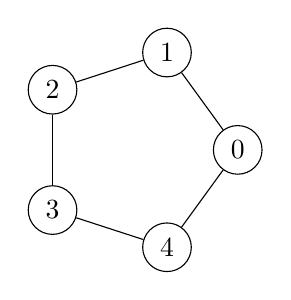
\begin{tikzpicture}
\foreach \i in {0, 1, 2, 3, 4}
   \node[circle, draw] (I\i) at (\i*72:1.3) {\i};
\foreach \i/\j in {0/1, 1/2, 2/3, 3/4, 4/0}
  \draw (I\i) -- (I\j);
\end{tikzpicture}\]
\end{minipage}
\end{Answer}
%-------------------------------------------------------------------------------
%-------------------------------------------------------------------------------
\begin{Exercise}\it
Écrire une fonction \type{est\_clique} telle que \type{est\_clique g xs} renvoie \type{true} si et seulement si la liste \type{xs} est une liste d'indices de sommets formant une clique dans le graphe
décrit par \type{g}.
\end{Exercise}  
%-------------------------------------------------------------------------------
\begin{lstlisting}
est_clique : int list array-> int list -> bool
\end{lstlisting}
%-------------------------------------------------------------------------------
\begin{Answer}
\begin{lstlisting}
let rec longueur liste =
  match liste with
  |[] -> 0
  |t::q -> 1 + longueur_liste q;;
 
let est_clique g xs =
   let p = longueur xs in
   let rec nb_voisins liste = 
      match liste with
      |[] -> 0
      |t::q -> if appartient xs t
               then 1 + nb_voisins q
               else nb_voisins q in
   let rec tester liste =
      match liste with
      |[] -> true
      |t::q -> (nb_voisins g.(t) = p-1) && tester q in
  tester xs;; 
\end{lstlisting} 
\end{Answer}
%-------------------------------------------------------------------------------
%-------------------------------------------------------------------------------
\section{Algorithme glouton pour la coloration}
%-------------------------------------------------------------------------------
%-------------------------------------------------------------------------------
Étant donnée une liste de segments $\overline{I}=(I_0,\dots,I_{n-1})$
de longueur $n\ge  1$, on se propose de déterminer une coloration
optimale de son graphe d'intervalles associé. 

On appelle coloration de $\overline{I}$ une coloration de $G\bigl(\overline I\bigr)$.

On suppose dans cette partie que les segments $I_k=[a_k,b_k]$, pour
$k\in \{0,\dots,n-1\}$, sont énumérés dans l'ordre croissant de leur
extrémités gauches, c'est-à-dire que $a_0\le a_1\le \dots\le a_{n-1}$.

On propose l'algorithme suivant :
\begin{lstlisting}
Pour k variant de 0 à n-1 
    colorer l'intervalle Ik 
        avec la plus petite couleur non encore utilisée 
        dans la coloration des intervalles Ij, 0 <= j < k,
        qui ont une intersection non vide avec Ik.
\end{lstlisting}
Ainsi, l'intervalle $I_0$ est toujours coloré avec la couleur 0,
l'intervalle $I_1$ reçoit la couleur $0$ si $I_0\cap I_1=\emptyset$,
et la couleur $1$ sinon, etc.
%-------------------------------------------------------------------------------
%-------------------------------------------------------------------------------
\begin{Exercise}[title=Un exemple]\it
Déterminer la coloration renvoyée par l'algorithme pour le problème (b).
\end{Exercise}  
%-------------------------------------------------------------------------------
\begin{Answer}

La numérotation des intervalles vérifie la propriété de croissance de l'extrémité gauche. 

On aboutit à la coloration (0, 1, 2, 0, 1, 0, 2, 1, 0).
\end{Answer}
%-------------------------------------------------------------------------------
%-------------------------------------------------------------------------------
\begin{Exercise}\it
Écrire une fonction \type{coloration} telle que l'appel \type{coloration seg}, où \type{seg} est un tableau contenant des segments triés par ordre croissant de leurs extrémités gauches, renvoie la coloration obtenue
avec l'algorithme ci-dessus.
\end{Exercise}  
%-------------------------------------------------------------------------------
\begin{lstlisting}
coloration : (int * int) array -> int list array-> int array
\end{lstlisting}
%-------------------------------------------------------------------------------
\begin{Answer}
On utilise les fonctions de la première partie.
\begin{lstlisting}
let coloration seg =
   let g = construit_graphe seg in
   let n = Array.length seg in
   let col = Array.make n (-1) in
   for i = 0 to (n-1) do 
      col.(i) <- couleur_disponible g col i done;
   col;;
\end{lstlisting} 
\end{Answer}
%-------------------------------------------------------------------------------
%-------------------------------------------------------------------------------
\subsection{Analyse}
%-------------------------------------------------------------------------------
%-------------------------------------------------------------------------------
On se propose maintenant de démontrer que l'algorithme ci-dessus fournit une coloration optimale de l'ensemble de segments. 
Soit $k$ un entier entre $0$ et $n-1$. On suppose qu'à la $k$-ième étape de
l'algorithme, le segment $I_k$ reçoit la couleur $c$.
%-------------------------------------------------------------------------------
%-------------------------------------------------------------------------------
\begin{Exercise}\it
L'extrémité gauche du segment $I_k$ appartient à un certain nombre de segments parmi $I_0,\dots,I_{k-1}$. Combien au moins~?
\end{Exercise}  
%-------------------------------------------------------------------------------
\begin{Answer}
Si $I_k$ a reçu la couleur $c$ alors il est lié avec des sommets qui on les couleurs 0 à $c-1$. Les seuls sommets colorés lors de la coloration de $I_k$ sont les sommets $I_0$ à $I_{k-1}$. Ainsi $I_k$ est lié avec au moins $c$ intervalles d'indices inférieurs à $k$. Or $I_k=[a_k;b_k]$ et $I_p=[a_p;b_p]$ sont liés si on a $a_k\in I_p$ ou $a_p\in I_k$. Pour $p\le k$ on a $a_p\le a_k$ donc les intervalles $I_p$ et $I_k$ sont en conflit si et seulement si $a_k\in I_p$.

Ainsi $a_k$ appartient à au moins $c$ intervalles d'indices inférieurs à $k$.
\end{Answer}
%-------------------------------------------------------------------------------
%-------------------------------------------------------------------------------
\begin{Exercise}[label=ques:clique]\it
Prouver que l'ensemble constitué de $I_k$ et de ses voisins d'indice inférieur à $k$ constitue une clique de taille au moins $c+1$ dans le graphe d'intervalles associé.
\end{Exercise}  
%-------------------------------------------------------------------------------
\begin{Answer}
On note $C$ l'ensemble des intervalles $I_p$ tels que $p\le k$ et $I_p\cap I_k \ne \emptyset$.
La question ci-dessus montre que $C$ contient au moins $c+1$ intervalles car il contient $I_k$ en plus de ses voisins.

Soient $I_p$ et $I_q$ appartenant à $C$. On a $a_k\in I_p$ et $a_k\in I_q$ donc $a_k\in I_p\cap I_q$ : $I_p\cap I_q\ne \emptyset$.

On en déduit que $(I_p,I_q)$ est une arête du graphe pour tous sommets $I_p$, $I_q$ de $C$ : $C$ est une clique de taille au moins $c+1$.
\end{Answer}
%-------------------------------------------------------------------------------
%-------------------------------------------------------------------------------
\begin{Exercise}[label=ques:min]\it
En déduire que le nombre de couleurs nécessaires à une coloration de l'ensemble des segments est au moins égal à $c+1$.
\end{Exercise}  
%-------------------------------------------------------------------------------
\begin{Answer}

La clique ci-dessus implique $\omega(G) \ge c+1$ donc, d'après la question \ref{ques:omega}, $\chi(G) \ge c+1$.
\end{Answer}
%-------------------------------------------------------------------------------
%-------------------------------------------------------------------------------
\begin{Exercise}[label=ques:opt]\it
Conclure.
\end{Exercise}  
%-------------------------------------------------------------------------------
\begin{Answer}
Lors de la coloration d'un sommet par une couleur $c$, toutes les couleurs de 0 à $c-1$ ont été attribuées à un sommet.
Si $c_M$ est la couleur maximale utilisée par l'algorithme, le nombre de couleurs utilisées est donc $c_M+1$. 
Ainsi $c_M+1 \ge \chi(G)$.

Lors de la coloration d'un sommet par $c_M$ la question ci-dessus montre qu'on a  $\chi(G) \ge c_M+1$.

On en déduit que $\chi(G) = c_M+1$ : la coloration de l'algorithme est optimale.
\end{Answer}
%-------------------------------------------------------------------------------
%-------------------------------------------------------------------------------
\begin{Exercise}[title=Complexité]\it
Déterminer la complexité de la fonction \type{coloration} en fonction du nombre $m$ d'arêtes du graphe d'intervalles associé à la liste $\overline{I}$.
\end{Exercise}  
%-------------------------------------------------------------------------------
\begin{Answer}
\begin{itemize}
\item La fonction \type{appartient} effectue au plus $p$ comparaisons où $p$ est la longueur de la liste passée en paramètre.
\item La fonction \type{plus\_petit\_absent} effectue au plus $c+1$ appels à \type{appartient} où $c$ est le résultat. Comme le nombre de couleurs est majoré par $p$, longueur de la liste, la complexité est majorée par $A.p.(p+1)$, c'est un ${\cal O}(p^2)$

\item La fonction \type{couleurs\_voisins} parcourt la liste des voisins d'un sommets, sa complexité est un ${\cal O}(m_i)$ où $m_i$ est le nombre de voisins de $i$, elle produit une liste de taille $m_i$ au plus.

\item Ainsi la fonction \type{couleur\_disponible} est de complexité en ${\cal O}(m_i^2)={\cal O}(m^2)$.

\item Enfin la fonction \type{coloration} fait appel $n$ fois à la fonction \type{couleur\_disponible} après avoir créé un tableau de taille $n$ où $n$ est le nombre de segments.

Sa complexité est donc un ${\cal O}(n + nm^2)$.
\end{itemize}

Il  semble difficile de donner une complexité ne faisant pas intervenir le nombre d'intervalles.
\end{Answer}
%-------------------------------------------------------------------------------
%-------------------------------------------------------------------------------
\section{Graphes munis d'un ordre d'élimination parfait}
%-------------------------------------------------------------------------------
%-------------------------------------------------------------------------------
Si $S'\subset S$ est un ensemble de sommets de $G$, le {\bf sous-graphe de $G$ induit par $S'$} est le
graphe $G' = (S',A')$ où $A'\subset A$ est l'ensemble des arêtes de $G$ dont les extrémités appartiennent à $S'$.

Soient $G = (S, A)$ un graphe et $(x_0,\dots,x_{n-1})$ une énumération
des sommets de $G$. 

Pour tout $i\in \{0,\dots,n-1\}$, on note $G_i=(S_i,A_i)$ sous-graphe de $G$ induit par $S_i=\{x_0,\dots,x_i\}$.

Une énumération $(x_0,\dots,x_{n-1})$ des sommets de $G$ est appelée
un {\bf ordre d'élimination parfait} si pour tout $i\in \{0,\dots,n-1\}$,
les voisins de $x_i$ d'indices inférieurs à $i$ forment une clique.
%--------------------------------------------------------------------------
\begin{figure}[ht]
\centering
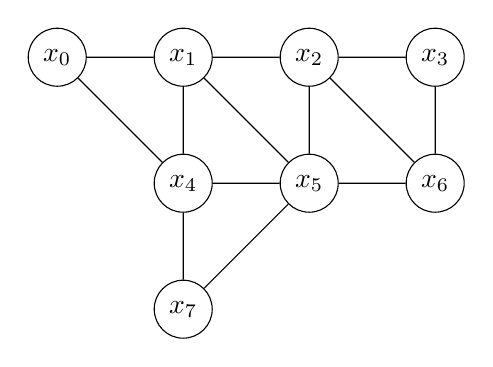
\begin{tikzpicture}[scale=0.8]
\foreach \k/\x/\y in {0/0/4, 1/2/4, 2/4/4, 3/6/4, 4/2/2, 5/4/2, 6/6/2, 7/2/0}
    \draw (\x, \y) node[draw,fill=white, circle] (x\k) {$x_\k$};
\foreach \i/\j in {0/1, 0/4, 1/2, 1/4, 1/5, 2/3, 2/5, 2/6, 3/6, 4/5, 4/7, 5/6, 5/7}
    \draw (x\i) -- (x\j);
\end{tikzpicture}
\caption{\label{fig:G0}Graphe $G_0$}
\end{figure} 
%-------------------------------------------------------------------------------
%-------------------------------------------------------------------------------
\begin{Exercise}[title=Un exemple]\it
Déterminer un ordre d'élimination parfait pour le graphe $G_0$ de la figure \ref{fig:G0}.
\end{Exercise}  
%-------------------------------------------------------------------------------
\begin{Answer}
L'ordre $(x_0, x_1, x_4, x_5, x_2, x_7, x_6, x_3)$ convient.

En effet les voisins  placés avant pour chaque sommet forment les ensembles

$\emptyset$, $\{x_0\}$, $\{x_0, x_1\}$,  $\{x_1, x_4\}$,  $\{x_1, x_5\}$,  $\{x_4, x_5\}$,   $\{x_2, x_5\}$ et  $\{x_2, x_6\}$ 

qui sont tous des cliques.  
\newpage
\end{Answer}
%-------------------------------------------------------------------------------
%-------------------------------------------------------------------------------
\subsection{Vérification}
%-------------------------------------------------------------------------------
%-------------------------------------------------------------------------------
\begin{Exercise}\it
Écrire une fonction \type{voisins\_inferieurs} telle que \type{voisins\_inferieurs g x} renvoie la liste des voisins du sommet d'indice $x$ dont l'indice est strictement inférieur à $x$.
\end{Exercise}  
%-------------------------------------------------------------------------------
\begin{lstlisting}
voisins_inferieurs : int list array-> int -> int list
\end{lstlisting}
%-------------------------------------------------------------------------------
\begin{Answer}
\begin{lstlisting}
let voisins_inferieurs g x =
   let rec aux liste = 
      match liste with
      |[] -> []
      |t::q when t < x -> t :: (aux q)
      |t::q -> aux q
  in aux g.(x);; 
\end{lstlisting}
\end{Answer}
%-------------------------------------------------------------------------------
%-------------------------------------------------------------------------------
\begin{Exercise}\it
Écrire une fonction \type{est\_ordre\_parfait} telle que \type{est\_ordre\_parfait g} renvoie \type{true} si et seulement si l'énumération associée au graphe représenté par \type{g} est un ordre d'élimination parfait.
\end{Exercise}  
%-------------------------------------------------------------------------------
\begin{lstlisting}
est_ordre_parfait : int list array-> bool
\end{lstlisting}
%-------------------------------------------------------------------------------
\begin{Answer}
\begin{lstlisting}
let est_ordre_parfait g =
   let n = Array.length g in
   let rec aux i =
      if i = n
      then true
      else let l = voisins_inferieurs g i in
           est_clique g l && aux (i+1)
  in aux 0;;
\end{lstlisting}
\end{Answer}
%-------------------------------------------------------------------------------
%-------------------------------------------------------------------------------
\begin{Exercise}[title = Cas des graphes d'intervalles]\it
Montrer que l'énumération des segments $(I_0,\dots,I_{n-1})$ obtenue en les triant par leurs extrémités gauches en ordre croissant est un ordre d'élimination parfait de leur graphe d'intervalles.
\end{Exercise}  
%-------------------------------------------------------------------------------
\begin{Answer}
L'ensemble des voisins de $I_k$ est l'ensemble des intervalles en conflit avec $I_k$. On a vu à la question \ref{ques:clique} que l'ensemble des voisins de $I_k$ d'ordre inférieur formaient une clique (la question ajoutait $I_k$ mais toute partie d'une clique est une clique).

On a donc bien un ordre d'élimination parfait.
\end{Answer}
%-------------------------------------------------------------------------------
\newpage
%-------------------------------------------------------------------------------
\subsection{Coloration}
%-------------------------------------------------------------------------------
%-------------------------------------------------------------------------------
On considère un graphe dont $(x_0,\dots,x_{n-1})$ est une énumération
des sommets. On colore ce graphe à l'aide l'algorithme suivant :
\begin{lstlisting}
Pour k variant de 0 à n-1 
    colorer le sommet xk 
    avec la plus petite couleur non encore utilisée 
    par un de ses voisins déjà colorés
\end{lstlisting}
%-------------------------------------------------------------------------------
%-------------------------------------------------------------------------------
\begin{Exercise}\it
Appliquer cet algorithme de coloration au graphe $G_0$ de la figure \ref{fig:G0} muni 
\begin{enumerate}
\item de l'ordre $(x_0,\dots,x_7)$,
\item d'un ordre d'élimination parfait.
\end{enumerate}
\end{Exercise}  
%-------------------------------------------------------------------------------
\begin{Answer}

\smallskip
{}\hfill
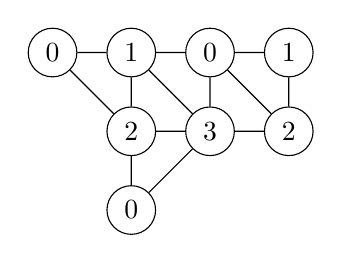
\begin{tikzpicture}
\node[circle, draw] (x0) at (0,0)  {0};
\node[circle, draw] (x1) at (1,0)  {1};
\node[circle, draw] (x2) at (2,0)  {0};
\node[circle, draw] (x3) at (3,0)  {1};
\node[circle, draw] (x4) at (1,-1) {2};
\node[circle, draw] (x5) at (2,-1) {3};
\node[circle, draw] (x6) at (3,-1) {2};
\node[circle, draw] (x7) at (1,-2) {0};
\draw (x0) -- (x1) -- (x2) -- (x3) -- (x6) -- (x5) -- (x7) -- (x4) -- (x0);
\draw (x5) -- (x4) -- (x1) -- (x5) -- (x2) -- (x6);
\end{tikzpicture}
\hfill
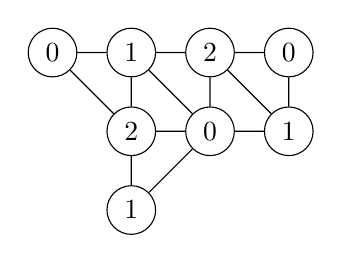
\begin{tikzpicture}
\node[circle, draw] (x0) at (0,0)  {0};
\node[circle, draw] (x1) at (1,0)  {1};
\node[circle, draw] (x2) at (2,0)  {2};
\node[circle, draw] (x3) at (3,0)  {0};
\node[circle, draw] (x4) at (1,-1) {2};
\node[circle, draw] (x5) at (2,-1) {0};
\node[circle, draw] (x6) at (3,-1) {1};
\node[circle, draw] (x7) at (1,-2) {1};
\draw (x0) -- (x1) -- (x2) -- (x3) -- (x6) -- (x5) -- (x7) -- (x4) -- (x0);
\draw (x5) -- (x4) -- (x1) -- (x5) -- (x2) -- (x6);
\end{tikzpicture}
\hfill{}
\end{Answer}
%-------------------------------------------------------------------------------
%-------------------------------------------------------------------------------
\begin{Exercise}\it
Soit $(c_0,\dots,c_{n-1})$ la coloration obtenue par cet
algorithme pour un graphe $G$ dont l'énumération des sommets est un
ordre d'élimination parfait.
\begin{enumerate}
\item  Montrer que pour tout $i\in \{0,\dots,n-1\}$, on a   $\chi(G)\ge  1+c_i$.
\item En déduire que l'algorithme de coloration renvoie une   coloration optimale.
\end{enumerate}
\end{Exercise}  
%-------------------------------------------------------------------------------
\begin{Answer}
On reprend les arguments des {\bf questions \ref{ques:min} et \ref{ques:opt}}.
\end{Answer}
%-------------------------------------------------------------------------------
%-------------------------------------------------------------------------------
\section{Ordre d'élimination parfait pour un graphe cordal}
%-------------------------------------------------------------------------------
%-------------------------------------------------------------------------------
Un graphe $G$ est dit {\bf cordal} lorsque pour tout cycle $C=(v_0,v_1,\dots,v_{n-1},v_0)$ de G de longueur $n\ge  4$, il existe $i,j$ distincts entre $0$ et $n-1$ tels que les sommets $v_i$ et $v_j$ soient reliés dans le graphe $G$ mais non successifs dans le cycle. Une telle arête $\{v_i,v_j\}$ est appelée une {\bf corde} du cycle C. Autrement dit, le graphe $G$ est cordal lorsque tout cycle de $G$ de longueur supérieure ou égale à 4 possède une corde.
%-------------------------------------------------------------------------------
%-------------------------------------------------------------------------------
\subsection{Cycles de longueur 4 dans un graphe d'intervalles}
%-------------------------------------------------------------------------------
%-------------------------------------------------------------------------------
Soit $G$ un graphe d'intervalles. 

Dans cette question, on se propose de démontrer par l'absurde que tout cycle de longueur $4$ de $G$ possède une corde. On suppose à cet effet que $G$ contient un $4$-cycle sans corde.

On dispose donc de quatre segments $I_0,I_1,I_2,I_3$ tels que 
\[I_0\cap I_1\ne \emptyset,\ I_1\cap I_2\ne \emptyset,\ I_2\cap I_3\ne \emptyset,\ I_3\cap I_0\ne \emptyset,\ I_0\cap I_2 = \emptyset,\ I_1\cap I_3 = \emptyset\]

On supposera pour simplifier que les extrémités des segments sont toutes distinctes.
%-------------------------------------------------------------------------------
%-------------------------------------------------------------------------------
\begin{Exercise}\it
Montrer qu'aucun des segments $I_k$, $k=0,1,2,3$, n'est inclus dans un autre de ces segments.
\end{Exercise}  
%-------------------------------------------------------------------------------
\begin{Answer}

Les intervalles jouent des rôles symétriques : supposons qu'on ait $I_0$ inclus dans $I_k$.

$I_0\subset I_2$ est impossible car $I_0\cap I_2=\emptyset$.

Si on a $I_0\subset I_1$ alors $I_0\cap I_3\subset I_1\subset I_3=\emptyset$ d'où $I_0\cap I_3 = \emptyset$, ce qui est impossible. 

De même $I_0\subset I_3$ est impossible.
\end{Answer}
%-------------------------------------------------------------------------------
%-------------------------------------------------------------------------------
\begin{Exercise}\it
On a donc par exemple $\min I_0 < \min I_1 < \max I_0 < \max I_1$. 

Montrer que $\min  I_1 < \min I_2 < \max I_1 < \max I_2$ et de même pour $I_2$ et $I_3$.
\end{Exercise}  
%-------------------------------------------------------------------------------
\begin{Answer}

On commence par démontrer la propriété admise.

Soient $I=[a;b]$ et $I'=[a';b']$ en conflit.

Pour $x\in I\cap I'$, on a $a\le x$ et $a'\le x$ donc $\max\{a, a'\}\le x$, de même $x\le \min\{b, b'\}$.

\begin{itemize}
    \item Si $\max\{a, a'\} = a$ et $\min\{b, b'\}=b$ alors $I=[a;b]\subset [a';b']=I'$.
    \item Si $\max\{a, a'\} = a$ et $\min\{b, b'\}=b'$ alors $a'\le a\le x\le b'\le b$.
    \item Si $\max\{a, a'\} = a'$ et $\min\{b, b'\}=b$  $a\le a'\le x\le b\le b'$.
    \item Si $\max\{a, a'\} = a'$ et $\min\{b, b'\}=b'$ alors $I'=[a';b']\subset [a;b]=I$.
\end{itemize}

Si on suppose de plus que les intervalles ne sont pas inclus l'un dans l'autre et que les extrémités sont toutes distinctes il ne reste que les possibilités
$a' < a < b' < b$ ou $a < a' < b < b'$.

\medskip

$I_0$ et $I_1$ sont en conflit, on suppose $a_0 < a_1 < b_0 < b_1$ : $I_0\cap I_1=[a_1; b_0]$.

$I_1$ et $I_2$ sont en conflit aussi, si on avait $a_2 < a_1 < b_2 < b_1$ alors on aurait $I_1\cap I_2=[a_1;b_2]$ donc $a_1\in I_2$, comme on avait aussi $a_1\in I_0$, on aboutit à $a_1\in I_0\cap I_2$, ce qui est impossible. 

On en déduit qu'on a $a_1< a_2< b_1< b_2$.

De même, on déduit de $I_2$ et $I_3$ en conflit qu'on a $a_2<a_3<b_2<b_3$.
\end{Answer}
%-------------------------------------------------------------------------------
%-------------------------------------------------------------------------------
\begin{Exercise}\it
Conclure à une contradiction.
\end{Exercise}  
%-------------------------------------------------------------------------------
\begin{Answer}
On déduit de la question précédente qu'on a $a_0<a_1<a_2<a_3$.

Comme $I_0$ et $I_3$ sont en conflits, cela impose $a_0<a_3<b_0<b_3$ donc $b_0\in I_3$.

Or an a aussi $I_0\cap I_1=[a_1; b_0]$ donc $b_0\in I_1$ on aboutit à $I_1\cap I_3\ne \emptyset$ ce qui est impossible.

\medskip

L'autre cas aboutit à une contradiction : il se ramène au premier cas en interchangeant $I_0$ et $I_1$ ainsi que $I_2$ et $I_3$.
\end{Answer}
%-------------------------------------------------------------------------------
%-------------------------------------------------------------------------------
\begin{Exercise}[title = Cordalité des graphes d'intervalles]\it
Montrer plus généralement que tout graphe d'intervalles est cordal.
\end{Exercise}  
%-------------------------------------------------------------------------------
\begin{Answer} La démonstration est la même. $I_0$, $I_1$, \ldots, $I_{p-1}$ est cycle : $p\ge 4$.

On suppose qu'on a $a_0 < a_1 < b_0 < b_1$ : $b_0\in I_0\cap I_1$.

Comme ci-dessus, si $(I_0, I_2)$ n'est pas une corde, on a $a_1< a_2< b_1< b_2$.

On peut poursuivre, si $(I_k, I_{k+2})$ n'est pas une corde, pour tout $k$ tel que $0\le k \le p-3$, on a 
$a_i<a_{i+1} < b_i < b_{i+1}$ pour tout $i$ tel que $0\le i \le p-2$.

Sous ces conditions on en déduit $a_0<a_{p-1}$ donc, comme $I_0$ et $I_{p-1}$ sont en conflit, $a_0<a_{p-1} < b_0 < b_{p-1}$. On conclut $b_0\in I_1\cap I_{p-1}$.

Il y a forcement une corde.
\end{Answer}
%-------------------------------------------------------------------------------
%-------------------------------------------------------------------------------
\subsection{Une enquête policière}
Six personnes sont entrées dans la bibliothèque le jour où un livre rare y a été volé. Chacune d'entre elles est entrée une seule fois dans la bibliothèque, y est restée un certain temps, puis elle en est sortie. Si deux personnes étaient ensemble dans la bibliothèque à un instant donné, alors au moins l'une des deux a vu l'autre. A l'issue de l'enquête, les témoignages recueillis sont les suivants : Albert dit
qu'il a vu Bernard et Edouard dans la bibliothèque. Bernard a vu Albert et Isabelle. Charlotte affirme avoir vu Didier et Isabelle. Didier dit qu'il a vu Albert et Isabelle. Edouard certifie avoir vu Bernard et Charlotte. Isabelle dit avoir vu Charlotte et Edouard. 
%-------------------------------------------------------------------------------
%-------------------------------------------------------------------------------
\begin{Exercise}\it
Seul le coupable a menti. Qui est-il~?
\end{Exercise}  
%-------------------------------------------------------------------------------
\begin{Answer}
On note $A,B,C,D,E,I$ les intervalles de temps de présence des différents protagonistes.

Les affirmations des personnes, si elles ne mentent pas, la vision (d'au moins) une personne par une autre caractérise les intervalles en conflit.

On aboutit au graphe
\[
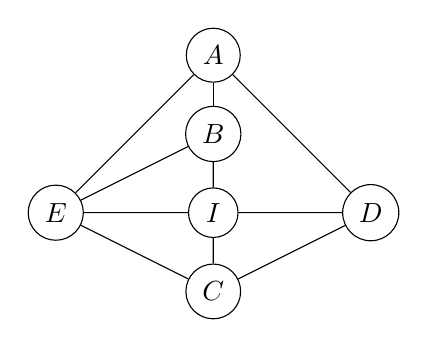
\begin{tikzpicture}
\node[circle, draw] (E) at (0,1) {$E$};
\node[circle, draw] (A) at (2,3) {$A$};
\node[circle, draw] (B) at (2,2) {$B$};
\node[circle, draw] (I) at (2,1) {$I$};
\node[circle, draw] (C) at (2,0) {$C$};
\node[circle, draw] (D) at (4,1) {$D$};
\draw (D) -- (C) -- (E) -- (I) -- (D) -- (A) -- (E) -- (B) -- (I) -- (C);
\draw (A) -- (B);
\end{tikzpicture}\]
On voit qu'il existe des cycle d'ordre 4 sans corde ce qui est impossible.

Les cycles sont $(A,D,I,B)$, $(A,D,I,E)$, $(A,D,C,E)$, 

Pour chacun de ces cycles, soit le cycle n'en est pas un, une des arêtes a été inventée soit il manque une corde, une des arêtes a été tue.
Dans les deux cas le menteur est une des personnes du cycle.


Le menteur doit donc être $A$ ou $D$.

Didier peut avoir menti en inventant avoir vu Albert.

Albert peut avoir menti et omis de dire qu'il a vu Isabelle et Charlotte.

On ne peut pas décider du coupable.
\end{Answer}
%-------------------------------------------------------------------------------
%-------------------------------------------------------------------------------
\subsection{Sommets simpliciaux}
%-------------------------------------------------------------------------------
%-------------------------------------------------------------------------------
Un sommet $v$ d'un graphe $G$ est {\bf simplicial} si l'ensemble
des voisins de $v$ dans $G$ est une clique.

On remarque que, si un graphe $G$ admet admet un ordre d'élimination parfait $(x_0, x_1, \ldots, x_{n-1})$; alors $x_{n-1}$ est simplicial car tous ses voisins sont d'indices inférieurs à $n-1$ et ils forment donc une clique.

\medskip

On représente en Caml le sous-graphe induit de $G$ induit par $S'$ par le couple \type{(g, sg)} de type \type{int list array
  * bool array} où \type{g} est une description du graphe $G$ et
\type{sg} est un tableau de booléens de taille $n$ tel que \type{sg.(i)} vaut \type{
  true} si et seulement si $i$ appartient à $S'$.
%-------------------------------------------------------------------------------
%-------------------------------------------------------------------------------
\begin{Exercise}\it
Écrire une fonction \type{simplicial} telle que l'appel \type{simplicial (g, sg) k}, où le sommet d'indice $k$ est supposé  appartenir au sous-graphe induit $G'$ décrit par \type{(g, sg)}, renvoie \type{true} si le sommet d'indice $k$ est simplicial dans $H$ et \type{false} sinon. 
Déterminer sa complexité.
\end{Exercise}  
%-------------------------------------------------------------------------------
\begin{lstlisting}
simplicial : (int list array * bool array) -> int -> bool
\end{lstlisting}
%-------------------------------------------------------------------------------
\begin{Answer}
Pour qu'un sommet soit simplicial il faut vérifier si l'ensemble de ses voisins appartenant à $H$ forme une clique dans $G'$, c'est-à-dire une clique dans $G$.

\begin{lstlisting}
let simplicial (g, sg) k =
   let rec extraire liste  =
      match liste with
      |[] -> []
      |t::q when sg.(t) -> t::(extraire q)
      |t::q -> extraire q in
   est_clique g (extraire g.(k));;
\end{lstlisting} 
Extraire les bons voisins se fait en parcourant la liste des voisins, de longueur $p$, sa complexité est donc un ${\cal O}(p)$.

Tester si un sous-ensemble forme un clique consiste, pour chaque élément, à compter le nombre de ses voisins dans l'ensemble : la complexité est donc un ${\cal O}(pn)$.

La complexité totale est donc un ${\cal O}\bigl(n^3\bigr)$ car on a $p\le n$.
\end{Answer}
%-------------------------------------------------------------------------------
%-------------------------------------------------------------------------------
\begin{Exercise}\it
Écrire une fonction \type{trouver\_simplicial} telle que l'appel \type{  trouver\_simplicial (g, sg)} renvoie, s'il en existe, un sommet simplicial du sous-graphe induit décrit par \type{(g, sg)}. 

Déterminer la complexité de cette fonction.
\end{Exercise}  
%-------------------------------------------------------------------------------
\begin{lstlisting}
trouver_simplicial : (int list array * bool array) -> int
\end{lstlisting}
%-------------------------------------------------------------------------------
\begin{Answer}
On choisit de renvoyer -1 s'il n'y a pas de sommet simplicial.
\begin{lstlisting}
let trouver_simplicial (g, sg) =
   let n = Array.length g in
   let simpl = ref (-1) in
   for k = 0 to (n-1) do
      if  sg.(k) && simplicial (g, sg) k
         then simpl := k done;
  !simpl;;
\end{lstlisting} 
On répète $n$ fois l'appel à simplicial : la complexité est un ${\cal O}\bigl(n^3\bigr)$.
\end{Answer}
%-------------------------------------------------------------------------------
%-------------------------------------------------------------------------------
\begin{Exercise}\it
$G$ admet un ordre d'élimination parfait $(x_0, x_1, \ldots, x_{n-1})$ et  $x_i$ est simplicial. 
Montrer que le graphe $G'$ induit par $\{x_0, \ldots, x_{i-1}, x_{i+1}, \ldots, x_{n-1}\}$ admet un ordre d'élimination parfait.
\end{Exercise}  
%-------------------------------------------------------------------------------
\begin{Answer}
On va prouver que $(x_0, \ldots, x_{i-1}, x_{i+1}, \ldots, x_{n-1})$ est un ordre d'élimination parfait.

On note $V'_k$ l'ensemble des voisins de $x_k$ d'indices inférieur à $k$ dans $G'$ et $V_k$ l'ensemble des voisins de $x_k$ d'indices inférieur à $k$ dans $G'$
\begin{itemize}
    \item Soit $V_k = V'_k$, dans ce cas $V_k$ forme une clique dans $G$ donc dans $G'$
    \item Soit $V_k = V'_k\cup \{x_i\}$, comme $V_k$ est une clique dans $G$, $V'_k$ en est une aussi donc c'est aussi une clique dans $G'$.
\end{itemize}
$(x_0, \ldots, x_{i-1}, x_{i+1}, \ldots, x_{n-1})$ est bien un ordre d'élimination parfait.\end{Answer}
%-------------------------------------------------------------------------------
%-------------------------------------------------------------------------------
\begin{Exercise}\it
Écrire une fonction \type{ordre\_parfait} telle que l'appel \type{ordre\_parfait  g} renvoie un ordre d'élimination parfait du graphe décrit par \type{g}, s'il en existe un. 

Déterminer la complexité de cette fonction.
\end{Exercise}  
%-------------------------------------------------------------------------------
\begin{lstlisting}
ordre_parfait : int list array -> int list
\end{lstlisting}
%-------------------------------------------------------------------------------
\begin{Answer}
Si $x$ est un sommet simplicial d'un graphe $G$ et si le sous-graphe $G'$ obtenu en supprimant $x$ admet un ordre d'élimination parfait alors $G$ admet un ordre d'élimination parfait obtenu en ajoutant $x$ à l'ordre d'élimination parfait dans $G'$.

Inversement si $G$ admet un ordre d'élimination parfait on sait qu'il admet un sommet simplicial et que le graphe induit en enlevant ce sommet admet un ordre d'élimination parfait.

On peut donc construire un  ordre d'élimination parfait récursivement :
\begin{itemize}
\item si le graphe est vide, son ordre d'élimination parfait est vide
    \item sinon, on détermine un sommet simplicial et on l'ajoute à un ordre d'élimination parfait du graphe induit en l'ôtant.
    
\end{itemize}
%--------------------------------------------------------------------------
\begin{lstlisting}
let ordre_parfait g =
   let n = Array.length g in
   let sg = Array.make n true in
   let rec aux_oep () =
      match trouver_simplicial (g, sg) with
      |-1 -> []
      |k -> sg.(k) <- false;
            k :: (aux_oep ()) in
   List.rev aux_oep ();;
\end{lstlisting} 
On cherche $n$ fois un simplicial : la complexité est un ${\cal O}\bigl(n^4\bigr)$
\end{Answer}
%-------------------------------------------------------------------------------
%-------------------------------------------------------------------------------
\subsection{Coupures minimales dans un graphe cordal}\label{part:cmin}
%-------------------------------------------------------------------------------
%-------------------------------------------------------------------------------
Étant donné un graphe $G$ on appelle {\bf coupure} de $G$ tout ensemble $C\subset S$ de sommets de $G$,% de cardinal au moins égal à $2$, 
tel que certains sommets reliés par un chemin dans le graphe $G$ ne le sont plus dans le sous-graphe $H$ de $G$ induit par $S\setminus C$.

On se donne dans cette question un graphe cordal $G = (S, A)$. 

Soient $C$ une coupure de $G$ de cardinal minimal % (supérieur ou égal à 2). 
et $H$ le sous-graphe de $G$ induit par $S\setminus C$. 

$a$ et $b$ sont deux sommets de $G$ déconnectés par la coupure, $S_1$ et $S_2$ sont les composantes connexes de $a$ et $b$ dans le graphe $H$ et $G_1$ et $G_2$ sont les graphes induits par $S_1$ et $S_2$. 
%-------------------------------------------------------------------------------
%-------------------------------------------------------------------------------
\begin{Exercise}\it
Montrer que tout point de $C$ est voisin dans $G$ d'un sommet de $S_1$ et d'un sommet de $S_2$.
\end{Exercise}  
%-------------------------------------------------------------------------------
\begin{Answer} 

On considère l'ensemble $C_1$ des sommet de $C$ qui sont voisins d'un sommet de $S_1$. 

Tout chemin $a\rightarrow s_1 \rightarrow \cdots \rightarrow s_{p-1} \rightarrow  b$ contient (au moins) un sommet de $C$. Le premier sommet de $C$ dans ce chemin est le successeur d'un sommet de $S_1$ donc appartient à $C_1$.

Ainsi toute chemin de $a$ vers $b$ contient un sommet de $C_1$ et $C_1$ est une coupure contenue dans $C$. Par minimalité de $C$ on en déduit qu'on a $C_1=C$. 

Tout sommet de $C$ est voisin d'un sommet de $S_1$.

De même tout sommet de $C$ est voisin d'un sommet de $S_2$.
\end{Answer}
%-------------------------------------------------------------------------------
%-------------------------------------------------------------------------------
$x$ et $y$ sont deux sommets distincts de $C$ (s'il en existe).
%-------------------------------------------------------------------------------
%-------------------------------------------------------------------------------
\begin{Exercise}\it
Montrer qu'il existe un chemin $P_1=(x,a_1,\dots,a_p,y)$ (resp. $P_2=(x,b_1,\dots,b_q,y)$) dont tous les sommets hormis $x$ et $y$ appartiennent à $S_1$ (resp. à $S_2$).
\end{Exercise}  
%-------------------------------------------------------------------------------
\begin{Answer}
On considère un voisin de $x$ dans $G_1$, $a'$, et un voisin de $y$ dans $G_1$, $a''$. $a'$ et $a''$ appartiennent à $S_1$ qui est une composante connexe du graphe induit donc il existe un chemin de $a'$ à $a'$ dans $G_1$ que l'on note $(a_1,a_2, \ldots,a_p)$.

Ainsi $(x, a_1,a_2, \ldots,a_p,y)$ est chemin de $G$ tel que demandé par l'énoncé.

De même il existe un chemin $(y, b_1,b_2, \ldots,b_q,x)$ dans $G$ avec $(b_1,b_2, \ldots,b_q)$ dans $G_2$.
\end{Answer}
%-------------------------------------------------------------------------------
%-------------------------------------------------------------------------------
\begin{Exercise}\it
On prend deux tels chemins $P_1$ et $P_2$ de longueur minimale. En considérant un cycle formé à partir des chemins $P_1$ et $P_2$, montrer que $x$ et $y$ sont voisins dans le graphe $G$.
\end{Exercise}  
%-------------------------------------------------------------------------------
\begin{Answer}
On trouve alors un cycle $(x, a_1,a_2, \ldots,a_p,y, b_1,b_2, \ldots,b_q,x)$ de longueur au moins $4$ dans $G$ qui est cordal.

Il admet donc une corde $(u,v)$. 
\begin{itemize}
\item Si $u\in G_1$ et $v\in G_1$ on écrit $u=a_i$ et $v=a_j$, on suppose $j\ge i+2$.

Si on remplace $(a_i,a_{i+1}, \ldots, a_j)$ par $(a_i,a_j)$, on obtient un cycle plus court avec les mêmes propriétés, ce qui est impossible.
\item De même il est impossible d'avoir $u\in G_2$ et $v\in G_2$.
\item La même démonstration montre qu'on ne peut pas avoir $u\in G_1$ ou $u\in G_2$ et $v=x$ ou $v=y$ ou l'inverse.
\end{itemize}
La seule possibilité est donc $(x,y) \in G$.
\end{Answer}
%-------------------------------------------------------------------------------
%-------------------------------------------------------------------------------
\begin{Exercise}\it
Montrer que $C$ est une clique du graphe $G$.
\end{Exercise}  
%-------------------------------------------------------------------------------
\begin{Answer}
Deux sommets quelconques de $C$ sont voisins dans $G$ donc $C$ est une clique de $G$.
\end{Answer}
%-------------------------------------------------------------------------------
%-------------------------------------------------------------------------------
\subsection{Sommets simpliciaux dans un graphe cordal}
%-------------------------------------------------------------------------------
%-------------------------------------------------------------------------------
On se propose de montrer la propriété ${\cal P}(G)$ : {\it tout graphe cordal $G$ possède un sommet simplicial, et même deux sommets  simpliciaux non voisins si $G$ n'est pas complet.} 

On se donne dans toute la suite un graphe cordal $G$.
%-------------------------------------------------------------------------------
%-------------------------------------------------------------------------------
\begin{Exercise}\it
Montrer que si $G$ est complet alors tous ses sommets sont simpliciaux.
\end{Exercise}  
%-------------------------------------------------------------------------------
\begin{Answer}
Dans un graphe complets tous ses sommets sont voisins donc toute partie est une clique. Ce sera le cas pour les voisins d'un sommet.
\end{Answer}
%-------------------------------------------------------------------------------
%-------------------------------------------------------------------------------
\begin{Exercise}\it
Montrer que la propriété ${\cal P}(G)$ est vérifiée si $G$ possède 1, 2 ou 3 sommets.
\end{Exercise}  
%-------------------------------------------------------------------------------
\begin{Answer}
\begin{enumerate}
\item Si $G$ possède un sommet, il est complet et son seul sommet est simplicial.
\item Si $G$ possède deux sommets, soit il est complet donc admet deux sommets simpliciaux soit il a deux sommets isolés qui sont simpliciaux et non adjacents.
\item Si $G$ possède deux sommets il admet de 0 à 3 arêtes.
\begin{enumerate}
  \item S'il n'admet aucune arête les 3 sommets sont simpliciaux et non adjacents.
  \item S'il admet 1 arête alors il y a un sommet isolé donc simplicial qui n'est pas voisins aux deux autres qui sont aussi simpliciaux.
  \item S'il admet 2 arêtes, le graphe est linéaire : $a_1$ est voisin de $a_2$ et $a_2$ est voisin de $a_3$.
  
  $a_1$ et $a_3$ sont alors simpliciaux et non voisins.
  \item S'il admet 3 arêtes, $G$ est complet : tous les sommets sont simpliciaux.
\end{enumerate}
\end{enumerate}
\end{Answer}
%-------------------------------------------------------------------------------
%-------------------------------------------------------------------------------
On suppose maintenant que $G$ n'est pas complet, possède au moins trois sommets et que la propriété ${\cal P}(G)$ est vérifiée pour tous les graphes cordaux $G'$ ayant strictement moins de sommets que $G$. 

On choisit une une coupure $C$ de $G$ de cardinal minimal. On a joute aux définitions de la partie \ref{part:cmin},  $H_1$ (resp $H_2$) est le sous-graphe de $G$ induit par $S_1\cup C$ (resp. par $S_2\cup C$).
%-------------------------------------------------------------------------------
%-------------------------------------------------------------------------------
\begin{Exercise}\it
Justifier que le graphe $H_1$ est cordal.
\end{Exercise}  
%-------------------------------------------------------------------------------
\begin{Answer}
\begin{lstlisting}
\end{lstlisting}
\end{Answer}
%-------------------------------------------------------------------------------
%-------------------------------------------------------------------------------
\begin{Exercise}\it
On suppose que $H_1$ est complet. Montrer que $S_1$ contient un sommet simplicial de $G$.
\end{Exercise}  
%-------------------------------------------------------------------------------
\begin{Answer}
Si $H_1$ est complet alors tout sommet de $S_1$ est simplicial pour $H_1$. Par exemple, $a$ l'est. Mais les voisins de $a$ dans $G$ sont tous soit dans $S_1$ soit dans $C$. $a$ est donc simplicial dans $G$.
\end{Answer}
%-------------------------------------------------------------------------------
%-------------------------------------------------------------------------------
\begin{Exercise}\it
On suppose que $H_1$ n'est pas complet. Montrer que $S_1\cup C$ contient deux sommets simpliciaux non voisins du graphe $H_1$. Montrer que au moins l'un de ces deux sommets est dans $S_1$ et que ce sommet est un sommet simplicial de $G$.
\end{Exercise}  
%-------------------------------------------------------------------------------
\begin{Answer}
Si $H_1$ n'est pas complet, par hypothèse de récurrence ${\cal P}(H_1)$ est vraie car $H_1$ n'a pas $b$ pour sommet. On peut trouver deux éléments de $S_1\cup C$ simpliciaux pour $H_1$ et non voisins dans $H_1$. Comme ils ne sont pas voisins et que $C$ est une clique, l'un des deux au moins est dans $S_1$. Comme ci-dessus, c'est alors un sommet simplicial de $G$.
\end{Answer}
%-------------------------------------------------------------------------------
%-------------------------------------------------------------------------------
\begin{Exercise}\it
Montrer que la propriété ${\cal P}(G)$ est vérifiée.
\end{Exercise}  
%-------------------------------------------------------------------------------
\begin{Answer}
Dans tous les cas on trouve un sommet simplicial de $G$ dans $S_1$ et de même on en trouve un dans $S_2$. Ces deux sommets ne peuvent pas être voisins dans $G$ car sinon on aurait un chemin de $a$ à $b$ ne passant pas par $C$. On a donc montré que ${\cal P}(G)$ est vérifiée. 

On a donc prouvé la récurrence sur la taille du graphe car la propriété est vraie pour les graphes de taille 3.
\end{Answer}
%-------------------------------------------------------------------------------
%-------------------------------------------------------------------------------
\begin{Exercise}\it
Montrer que tout graphe cordal possède un ordre d'élimination
% parfait.
\end{Exercise}  
%-------------------------------------------------------------------------------
\begin{Answer}
Tout graphe cordal $G$ admet au moins un sommet simplicial $x$. 

Le graphe induit par $S\setminus\{x\}$, $H$, est encore cordal.

Par récurrence sur la taille on peut construire une suite de sommets qui créent  un ordre d'élimination parfait.
\end{Answer}
%-------------------------------------------------------------------------------
%-------------------------------------------------------------------------------
